\item {\bf Sampling}

\begin{center}
  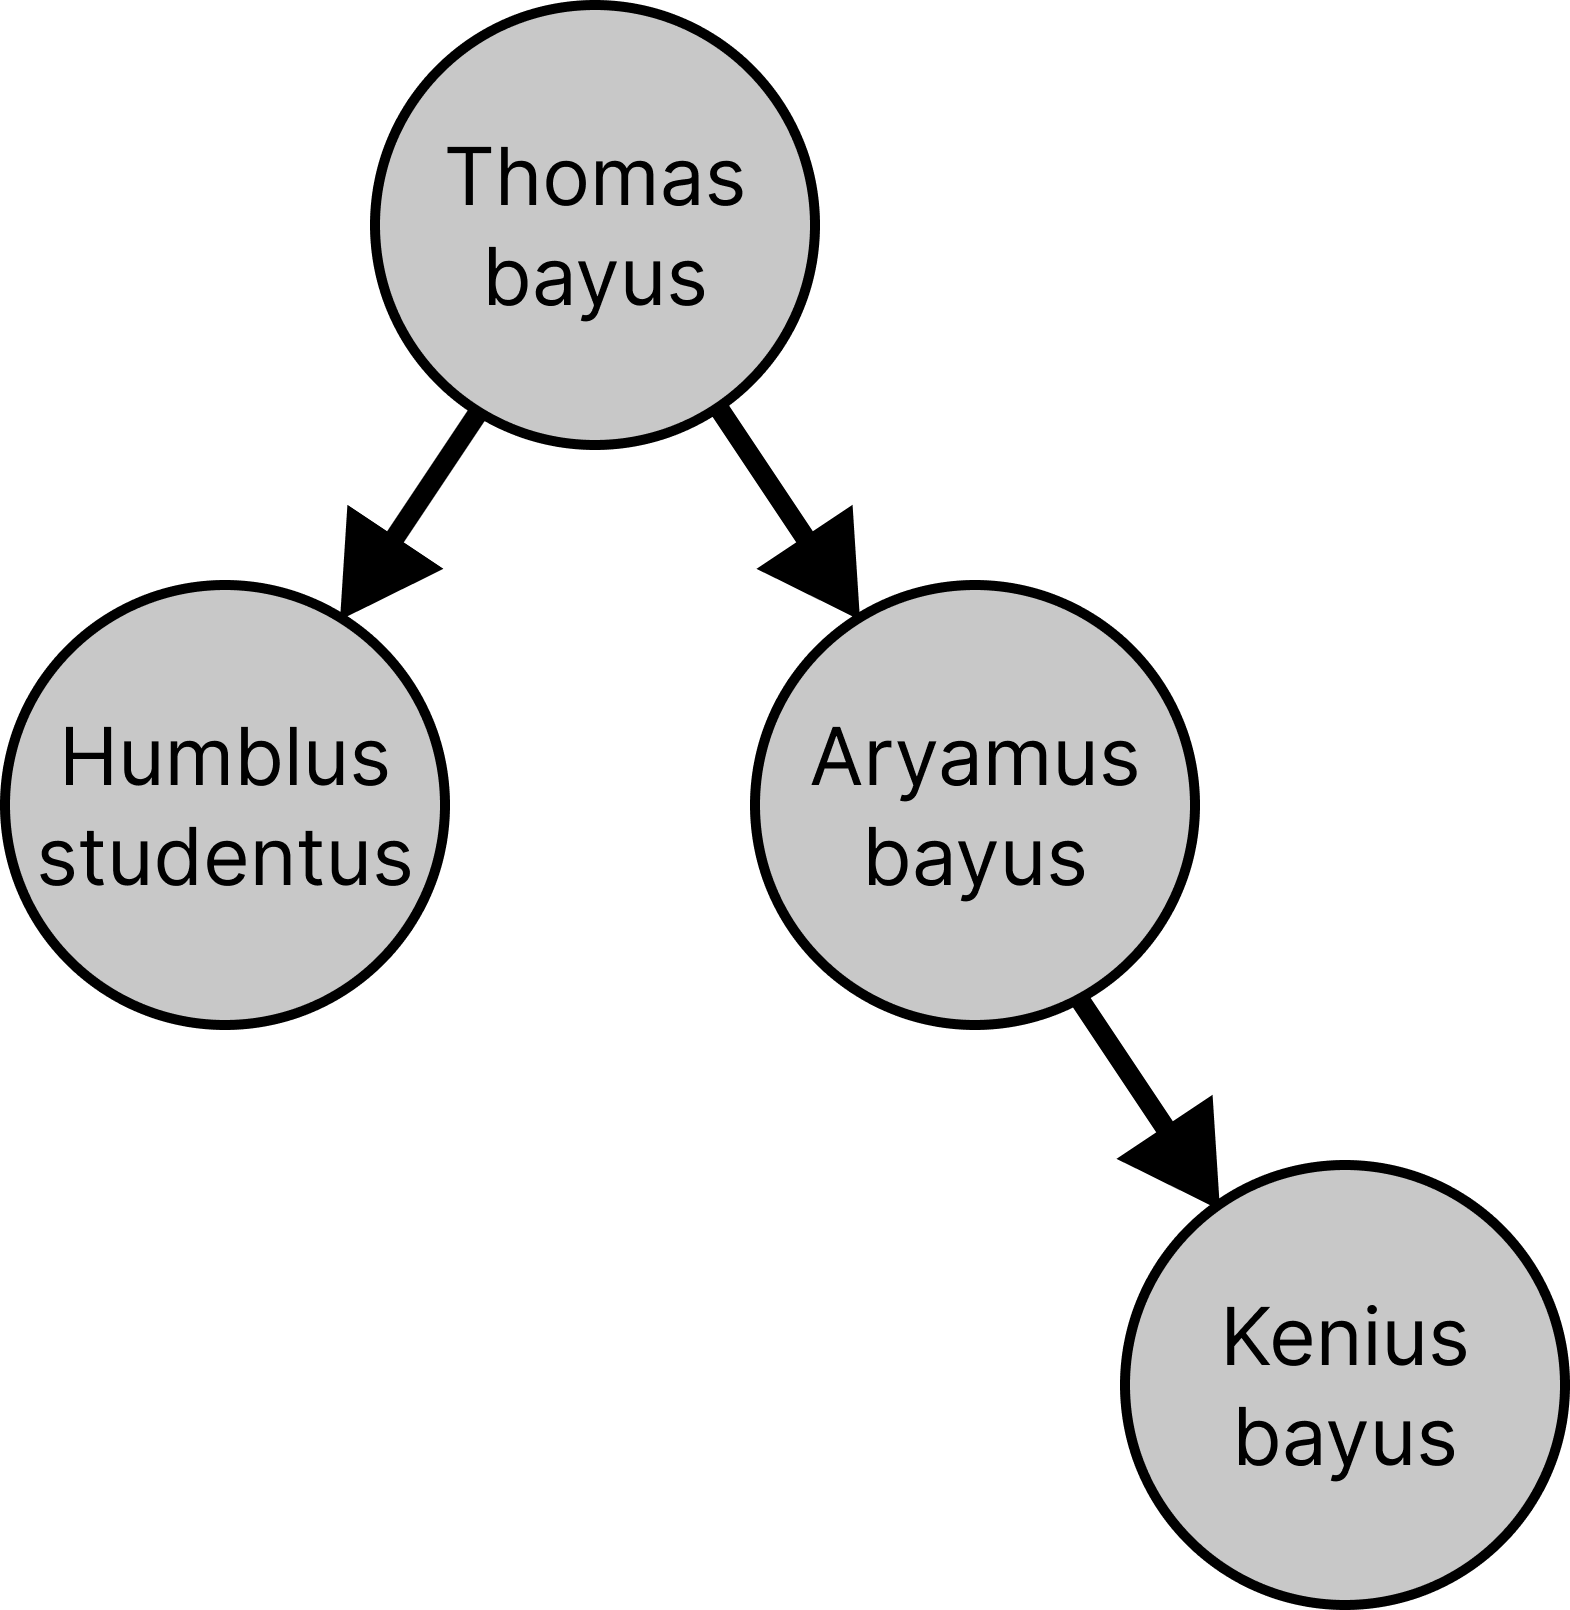
\includegraphics[width=0.5\textwidth]{images/dna.png}
\end{center}

You got distracted while examining that luscious green grass in the Stanford Oval, and you somehow wandered into the Gilbert Biological Sciences Building. As you realize where you are, you overhear some biologists discussing the genome of a new species they've discovered, provisionally given the scientific name \textit{Kenius bayus}.

(As you remember from high school biology, the genome of a living thing is encoded in DNA, which is a long chain of nucleotides. Each nucleotide can be one of four organic molecules: \textit{A}, \textit{C}, \textit{T}, or \textit{G}.)

Assume a simplified model of biology where each descendant mutates the gene of its ancestor with a probability of \texttt{mutation\_rate}, with a uniform distribution over the other three nucleotides when mutating. The mutation process is independent for each nucleotide.

For example, if we set \texttt{mutation\_rate = 0.1}, then the local conditional probability table for $p(\text{HumblusStudentus} \mid \text{ThomasBayus})$ would be:

\begin{center}
\lstDeleteShortInline|
\begin{tabular}{|c|c|c|c|c|}
\hline
$\text{ThomasBayus}$ & $p(\text{HS} = \text{A} \mid \text{TB})$ & $p(\text{HS} = \text{C} \mid \text{TB})$ & $p(\text{HS} = \text{T} \mid \text{TB})$ & $p(\text{HS} = \text{G} \mid \text{TB})$ \\
\hline
$\text{A}$ & $0.9$ & $0.03333$ & $0.03333$ & $0.03333$ \\
$\text{C}$ & $0.03333$ & $0.9$ & $0.03333$ & $0.03333$ \\
$\text{T}$ & $0.03333$ & $0.03333$ & $0.9$ & $0.03333$ \\
$\text{G}$ & $0.03333$ & $0.03333$ & $0.03333$ & $0.9$ \\
\hline
\end{tabular}
\lstMakeShortInline|
\end{center}

The biologists are trying to figure out the probability of \textit{Kenius bayus}'s genome resulting from a series of mutations from its ancestor, \textit{Thomas bayus}. You realise you could help these poor biologists, who never took CS 221, by modelling the mutation process with Bayesian networks!

\begin{enumerate}

  \item \points{2a}
Let's first get familiar with the provided interface for Bayesian networks. Convert the provided phylogenetic tree into a Bayesian network using the \texttt{BayesianNetwork} class and the \texttt{BayesianNode} class defined in \texttt{util.py}.

\begin{redbox}

  \textbf{Understanding the shape of the conditional probability table (CPT):} When you create a \texttt{BayesianNode}, the last dimension of its conditional probability table will correspond to that node's domain, and every preceding dimension will match the size of each parent's domain (in parent order). For example, a node with two parents whose domains are length 4 and a child domain of length 4 needs a CPT of shape \texttt{(4, 4, 4)}.

  By default, the \texttt{BayesianNode} constructor will create a uniform distribution over the domain, but for some problems you may need to set the CPTs to a different distribution.

  \textbf{For later problems:} Remember to read and understand the member functions of the \texttt{BayesianNode} class in \texttt{util.py}, particularly \texttt{get\_probability}, \texttt{parent\_assignment\_indices}, and \texttt{iter\_parent\_assignments}.

  Also, each \texttt{BayesianNetwork} has a \texttt{batch\_size} parameter, which sets the size of a special batch axis for the nodes without parents. Your code may have to handle such nodes as a special case. This batch axis is used to sample sequences of independent observations (e.g. perhaps a DNA sequence...). By default, the \texttt{batch\_size} is 1, but for some problems you may need to set it to a different value.

\end{redbox}


\expect{
  An implementation of the \texttt{initialize\_phylogenetic\_tree} function in \texttt{submission.py}, which takes in a \texttt{mutation\_rate} and returns a \texttt{BayesianNetwork} object representing the phylogenetic tree with the conditional probability tables being determined by the mutation rate.

  We provide code for varying the \texttt{genome\_length} parameter; you only need to define each node and its domain, parents, and conditional probability table.
}
  \item \points{2b}

You will need to implement some initial scaffolding to enable sampling from Bayesian networks in the code.
Extend the \texttt{BayesianNetwork} class and implement the function \texttt{forward\_sampling}. This function should sample a single observation from the joint probability distribution of the given Bayesian network.

\expect{
    An implementation of the \texttt{forward\_sampling} function in \texttt{submission.py}. You should use the given ordering of variables in \texttt{self.order} and sample from each one in order, using its conditional probability distribution and the values of its parents (which you should have already sampled). Each variable is represented by a \texttt{BayesianNode} object. Your solution should explicitly handle varying sequence lengths by using the \texttt{network.batch\_size} parameter.
}
  \item \points{2c}

Implement \texttt{compute\_joint\_probability}, which computes the joint probability of a given set of assignments to the variables in the Bayesian network.

\expect{
An implementation of the \texttt{compute\_joint\_probability} function in \texttt{submission.py}. Your solution should explicitly handle varying sequence lengths by using the \texttt{network.batch\_size} parameter.
}
  \input{02-sampling/04-genome}
  \item \points{2e}

Now we will use \textbf{rejection sampling} to estimate the following posterior probability: $\mathbb{P}(\text{ThomasBayus} = \text{AAAC} \mid \text{KeniusBayus} = \text{AAAA})$.

Implement the function \texttt{rejection\_sampling}, which takes in a setting for \textit{Kenius bayus}'s gene (as a list of nucleotide strings, e.g. \texttt{['A', 'A', 'A', 'A']}) along with the number of samples as an argument.

\expect{
    An implementation of the \texttt{rejection\_sampling} function in \texttt{submission.py}. Your implementation should directly call the \texttt{forward\_sampling} function you implemented in part (b). As before, your solution should explicitly handle the sequence length dimension by using the \texttt{network.batch\_size} parameter.
}
  \item \points{2f}

We will now implement \textbf{Gibbs sampling} because these biologists are getting impatient. Complete the implementation of the iteration loop in the \texttt{gibbs\_sampling} function, which takes in a dictionary with settings for the evidence variables along with number of iterations. We have implemented the initial assignment for you.

\expect{
    An implementation of the iteration loop in the \texttt{gibbs\_sampling} function in \texttt{submission.py}.
}

  \input{02-sampling/07-sampling-comparison}

\end{enumerate}
